%
% parrondo.tex -- Anwendung: analyse von Parrondos Paradoxon
%
% (c) 2020 Prof Dr Andreas Müller, Hochschule Rapperswil
%
\section{Das Paradoxon von Parrondo
\label{buch:section:paradoxon-von-parrondo}}
\rhead{Das Paradoxon von Parrondo}
Das Paradoxon von Parrondo ist ein der Intuition widersprechendes
Beispiel für eine Kombination von Spielen mit negativer Gewinnerwartung,
deren Kombination zu einem Spiel mit positiver Gewinnerwartung führt.
Die Theorie der Markov-Ketten und der zugehörigen Matrizen ermöglicht
eine sehr einfache Analyse.

%
% Parrondo Teilspiele
%
\subsection{Die beiden Teilspiele
\label{buch:subsection:teilspiele}}

\subsubsection{Das Spiel $A$}
Das Spiel $A$ besteht darin, eine Münze zu werfen.
Je nach Ausgang gewinnt oder verliert der Spieler eine Einheit.
Sei $X$ die Zufallsvariable, die den gewonnen Betrag beschreibt.
Für eine faire Münze ist die Gewinnerwartung in diesem Spiel natürlich
$E(X)=0$.
Wenn die Wahrscheinlichkeit für einen Gewinn $\frac12+e$ ist, dann muss
die Wahrscheinlichkeit für einen Verlust $\frac12-e$ sein, und die 
Gewinnerwartung ist
\(
E(X)
=
1\cdot P(X=1) + (-1)\cdot P(X=-1)
=
\frac12+e + (-1)\biggl(\frac12-e\biggr)
=
2e.
\)
Die Gewinnerwartung ist also genau dann negativ, wenn $e<0$ ist.

\subsubsection{Das Spiel $B$}
Das zweite Spiel $B$ ist etwas komplizierter, da der Spielablauf vom 
aktuellen Kapital $K$ des Spielers abhängt.
Wieder gewinnt oder verliert der Spieler eine Einheit,
die Gewinnwahrscheinlichkeit hängt aber vom Dreierrest des Kapitals ab.
Sei $Y$ die Zufallsvariable, die den Gewinn beschreibt.
Ist $K$ durch drei teilbar, ist die Gewinnwahrscheinlichkeit $\frac1{10}$,
andernfalls ist sie $\frac34$.
Formell ist
\begin{equation}
\begin{aligned}
P(Y=1|\text{$K$ durch $3$ teilbar}) &=  \frac{1}{10}
\\
P(Y=1|\text{$K$ nicht durch $3$ teilbar}) &= \frac{3}{4}
\end{aligned}
\label{buch:wahrscheinlichkeit:eqn:Bwahrscheinlichkeiten}
\end{equation}
Insbesondere ist die Wahrscheinlichkeit für einen Gewinn in zwei der
Fälle recht gross, in einem Fall aber sehr klein.

\subsubsection{Übergangsmatrix im Spiel $B$}
\begin{figure}
\centering
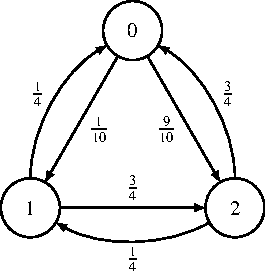
\includegraphics{chapters/80-wahrscheinlichkeit/images/spielB.pdf}
\caption{Zustandsdiagramm für das Spiel $B$, Zustände sind die
Dreierreste des Kapitals.
\label{buch:wahrscheinlichkeit:fig:spielB}}
\end{figure}%
Für den Verlauf des Spiels spielt nur der Dreierrest des Kapitals
eine Rolle.
Es gibt daher drei mögliche Zustände $0$, $1$ und $2$.
In einem Spielzug finde ein Übergang in einen anderen Zustand
statt, der Eintrag $b_{ij}$ ist die Wahrscheinlichkeit
\[
b_{ij}
=
P(K\equiv i|K\equiv j),
\]
dass ein Übergang vom Zustand $j$ in den Zustand $i$ stattfindet.
Die Matrix ist
\[
B=
\begin{pmatrix}
0          &\frac14 &\frac34\\
\frac1{10} &0       &\frac14\\
\frac9{10} &\frac34 &0
\end{pmatrix}.
\]

\subsubsection{Gewinnerwartung in einem Einzelspiel $B$}
Die Gewinnerwartung einer einzelnen Runde des Spiels $B$ hängt natürlich
ebenfalls vom Ausgangskapital ab.
Mit den Wahrscheinlichkeiten von 
\eqref{buch:wahrscheinlichkeit:eqn:Bwahrscheinlichkeiten}
findet man die Gewinnerwartung
\begin{equation}
\begin{aligned}
E(Y| \text{$K$ durch $3$ teilbar})
&=
1\cdot P(Y=1|K\equiv 0\mod 3)
+
(-1)\cdot P(Y=-1|K\equiv 0\mod 3)
\\
&=
\frac1{10}
-
\frac{9}{10}
=
-\frac{8}{10}
\\
E(Y| \text{$K$ nicht durch $3$ teilbar})
&=
1\cdot P(Y=1|K\not\equiv 0\mod 3)
+
(-1)\cdot P(Y=-1|K\not\equiv 0\mod 3)
\\
&=
\frac34-\frac14
=
\frac12.
\end{aligned}
\label{buch:wahrscheinlichkeit:eqn:Berwartungen}
\end{equation}
Falls $K$ durch drei teilbar ist, muss der Spieler
also mit einem grossen Verlust rechnen, andernfalls mit einem
moderaten Gewinn.

Ohne weiteres Wissen über das Anfangskapital ist es zulässig anzunehmen,
dass die drei möglichen Reste die gleiche Wahrscheinlichkeit haben.
Die Gewinnerwartung in diesem Fall ist dann
\begin{align}
E(Y)
&=
E(Y|\text{$K$ durch $3$ teilbar}) \cdot \frac13
+
E(Y|\text{$K$ nicht durch $3$ teilbar}) \cdot \frac23
\notag
\\
&=
-\frac{8}{10}\cdot\frac{1}{3}
+
\frac{1}{2}\cdot\frac{2}{3}
=
-\frac{8}{30}+\frac{10}{30}
=
\frac{2}{30}
=
\frac{1}{15}.
\label{buch:wahrscheinlichkeit:eqn:Beinzelerwartung}
\end{align}
Unter der Annahme, dass alle Reste die gleiche Wahrscheinlichkeit haben,
ist das Spiel also ein Gewinnspiel.

Die Berechnung der Gewinnerwartung in einem Einzelspiel kann man 
wie folgt formalisieren.
Die Matrix $B$ gibt die Übergangswahrscheinlichkeiten zwischen
verschiedenen Zuständen.
Die Matrix 
\[
G=\begin{pmatrix}
 0&-1& 1\\
 1& 0&-1\\
-1& 1& 0
\end{pmatrix}
\]
gibt die Gewinne an, die bei einem Übergang anfallen.
Die Matrixelemente $g_{ij}b_{ij}$ des Hadamard-Produktes 
$G\odot B$
von $G$ mit $B$ enthält in den Spalten die Gewinnerwartungen
für die einzelnen Übergänge aus einem Zustand.
Die Summe der Elemente der Spalte $j$ enthält die Gewinnerwartung
\[
E(Y|K\equiv j)
=
\sum_{i=0}^2 g_{ij}b_{ij}
\]
für einen Übergang aus dem Zustand $j$.
Man kann dies auch als einen Zeilenvektor schreiben, der durch Multiplikation
der Matrix $G\odot B$ mit dem Zeilenvektor
$U^t=\begin{pmatrix}1&1&1\end{pmatrix}$
entsteht:
\[
\begin{pmatrix}
E(Y|K\equiv 0)&
E(Y|K\equiv 1)&
E(Y|K\equiv 2)
\end{pmatrix}
=
U^t
G\odot B.
\]
Die Gewinnerwartung ist dann das Produkt
\[
E(Y)
=
\sum_{i=0}^2
E(Y|K\equiv i) p_i
=
U^t
(G\odot B)p.
\]
Tatsächlich ist
\[
G\odot B
=
\begin{pmatrix}
 0          &-\frac14 & \frac34\\
 \frac1{10} & 0       &-\frac14\\
-\frac9{10} & \frac34 & 0
\end{pmatrix}
\quad\text{und}\quad
U^t G\odot B
=
\begin{pmatrix}-\frac{8}{10}&\frac12&\frac12\end{pmatrix}.
\]
Dies stimmt mit den Erwartungswerten in 
\eqref{buch:wahrscheinlichkeit:eqn:Berwartungen}
überein.
Die gesamte Geinnerwartung ist dann
\begin{equation}
(G\odot B)
\begin{pmatrix}\frac13\\\frac13\\\frac13\end{pmatrix}
=
\begin{pmatrix}-\frac{8}{10}&\frac12&\frac12\end{pmatrix}
\frac13U
=
\frac13\biggl(-\frac{8}{10}+\frac12+\frac12\biggr)
=
\frac13\cdot\frac{2}{10}
=
\frac{1}{15},
\label{buch:wahrscheinlichkeit:eqn:BodotEinzelerwartung}
\end{equation}
dies stimmt mit \eqref{buch:wahrscheinlichkeit:eqn:Beinzelerwartung}
überrein.

\subsubsection{Das wiederholte Spiel $B$}
Natürlich spielt man das Spiel nicht nur einmal, sondern man wiederholt es.
Es ist verlockend anzunehmen, dass die Dreierreste $0$, $1$ und $2$ des
Kapitals immer noch gleich wahrscheinlich sind.
Dies braucht jedoch nicht so zu sein.
Wir prüfen die Hypothese daher, indem wir die Wahrscheinlichkeit
für die verschiedenen Dreierreste des Kapitals in einem interierten
Spiels ausrechnen.

Das Spiel kennt die Dreierreste als die drei für das Spiel ausschlaggebenden
Zuständen.
Das Zustandsdiagramm~\ref{buch:wahrscheinlichkeit:fig:spielB} zeigt
die möglichen Übergänge und ihre Wahrscheinlichkeiten, die zugehörige
Matrix ist
\[
B
=
\begin{pmatrix}
0          &\frac14 &\frac34\\
\frac1{10} &0       &\frac14\\
\frac9{10} &\frac34 &0
\end{pmatrix}
\]
Die Matrix $B$ ist nicht negativ und man kann nachrechnen, dass $B^2>0$ ist.
Damit ist die Perron-Frobenius-Theorie von
Abschnitt~\ref{buch:section:positive-vektoren-und-matrizen}
anwendbar.

Ein Eigenvektor zum Eigenwert $1$ kann mit Hilfe des Gauss-Algorithmus
gefunden werden:
\begin{align*}
\begin{tabular}{|>{$}c<{$}>{$}c<{$}>{$}c<{$}|}
\hline
-1         &\frac14 &\frac34 \\
\frac1{10} &-1      &\frac14 \\
\frac9{10} &\frac34 &-1      \\
\hline
\end{tabular}
&\rightarrow
\begin{tabular}{|>{$}c<{$}>{$}c<{$}>{$}c<{$}|}
\hline
1          &-\frac14       &-\frac34       \\
0          &-\frac{39}{40} & \frac{13}{40} \\
0          & \frac{39}{40} &-\frac{13}{40} \\
\hline
\end{tabular}
\rightarrow
\begin{tabular}{|>{$}c<{$}>{$}c<{$}>{$}c<{$}|}
\hline
1 &-\frac14 &-\frac34 \\
0 & 1       &-\frac13 \\
0 & 0       & 0       \\
\hline
\end{tabular}
\rightarrow
\begin{tabular}{|>{$}c<{$}>{$}c<{$}>{$}c<{$}|}
\hline
1 & 0 &-\frac56 \\
0 & 1 &-\frac13 \\
0 & 0 & 0       \\
\hline
\end{tabular}
\end{align*}
Daraus liest man einen möglichen Lösungsvektor mit den Komponenten
$5$, $2$ und $6$ ab.
Wir suchen aber einen Eigenvektor, der als Wahrscheinlichkeitsverteilung
dienen kann.
Dazu müssen sich die Komponente zu $1$ summieren, was man durch normieren
in der $l^1$-Norm erreichen kann:
\begin{equation}
p
=
\begin{pmatrix}
P(K\equiv 0)\\
P(K\equiv 1)\\
P(K\equiv 2)
\end{pmatrix}
=
\frac{1}{5+2+6}
\begin{pmatrix}
5\\2\\6
\end{pmatrix}
=
\frac{1}{13}
\begin{pmatrix}
5\\2\\6
\end{pmatrix}
\approx
\begin{pmatrix}
   0.3846 \\
   0.1538 \\
   0.4615
\end{pmatrix}.
\label{buch:wahrscheinlichkeit:spielBP}
\end{equation}
Die Hypothese, dass die drei Reste gleich wahrscheinlich sind, ist
also nicht zutreffend.

Die Perron-Frobenius-Theorie sagt, dass sich die
Verteilung~\ref{buch:wahrscheinlichkeit:spielBP} nach einiger Zeit
einstellt.
Wir können jetzt auch die Gewinnerwartung in einer einzelnen 
Runde des Spiels ausgehend von dieser Verteilung der Reste des Kapitals
berechnen.
Dazu brauchen wir zunächst die Wahrscheinlichkeiten für Gewinn oder
Verlust, die wir mit dem Satz über die totale Wahrscheinlichkeit 
nach
\begin{align*}
P(Y=+1)
&=
P(Y=+1|K\equiv 0) \cdot P(K\equiv 0)
+
P(Y=+1|K\equiv 1) \cdot P(K\equiv 1)
+
P(Y=+1|K\equiv 2) \cdot P(K\equiv 2)
\\
&=
\frac{1}{10}\cdot\frac{5}{13}
+
\frac{3}{4} \cdot\frac{2}{13}
+
\frac{3}{4} \cdot\frac{6}{13}
\\
&=
\frac1{13}\biggl(
\frac{1}{2}+\frac{3}{2}+\frac{9}{2}
\biggr)
=
\frac{13}{26}
=
\frac12
\\
P(Y=-1)
&=
P(Y=-1|K\equiv 0) \cdot P(K\equiv 0)
+
P(Y=-1|K\equiv 1) \cdot P(K\equiv 1)
+
P(Y=-1|K\equiv 2) \cdot P(K\equiv 2)
\\
&=
\frac{9}{10}\cdot\frac{5}{13}
+
\frac{1}{4} \cdot\frac{2}{13}
+
\frac{1}{4} \cdot\frac{6}{13}
\\
&=
\frac{1}{13}\biggl(
\frac{9}{2} + \frac{1}{2} + \frac{3}{2}
\biggr)
=
\frac{1}{2}
\end{align*}
berechnen können.
Gewinn und Verlust sind also gleich wahrscheinlich, das Spiel $B$ ist also
ebenfalls fair.

Auch diese Gewinnwahrscheinlichkeit kann etwas formeller mit dem
Hadamard-Produkt berechnet werden:
\[
U^t (G\odot B) p
=
\begin{pmatrix}-\frac{8}{10}&\frac12&\frac12\end{pmatrix}
\frac{1}{13}
\begin{pmatrix}
5\\2\\6
\end{pmatrix}
=
-\frac{8}{10}\cdot\frac{5}{13}
+\frac{1}{2} \cdot\frac{2}{13}
+\frac{1}{2} \cdot\frac{6}{13}
=
\frac{1}{26}(-8 + 2+ 6)
=
0,
\]
wie erwartet.

\subsubsection{Das modifizierte Spiel $\tilde{B}$}
\begin{figure}
\centering
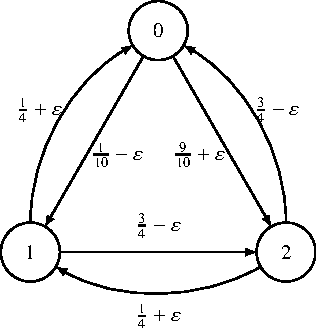
\includegraphics{chapters/80-wahrscheinlichkeit/images/spielBtilde.pdf}
\caption{Zustandsdiagramm für das modifizerte Spiel $\tilde{B}$,
Zustände sind die Dreierreste des Kapitals.
Gegenüber dem Spiel $B$
(Abbildung~\ref{buch:wahrscheinlichkeit:fig:spielB})
sind die Wahrscheinlichkeiten für Verlust 
um $\varepsilon$ vergrössert und die Wahrscheinlichkeiten für Gewinn um
$\varepsilon$ verkleinert worden.
\label{buch:wahrscheinlichkeit:fig:spielBtile}}
\end{figure}
%
Wir modifizieren jetzt das Spiel $B$ derart, dass die Wahrscheinlichkeiten
für Gewinn um $\varepsilon$ verringert werden und die Wahrscheinlichkeiten
für Verlust um $\varepsilon$ vergrössert werden.
Die Übergangsmatrix des modifzierten Spiels $\tilde{B}$ ist
\[
\tilde{B}
=
\begin{pmatrix}
 0                       & \frac{1}{4}+\varepsilon & \frac{3}{4}-\varepsilon \\
\frac{1}{10}-\varepsilon & 0                       & \frac{1}{4}+\varepsilon \\
\frac{9}{10}+\varepsilon & \frac{3}{4}-\varepsilon & 0
\end{pmatrix}
=
B
+
\varepsilon
\underbrace{
\begin{pmatrix}
 0& 1&-1\\
-1& 0& 1\\
 1&-1& 0
\end{pmatrix}
}_{\displaystyle F}
\]
Wir wissen bereits, dass der Vektor $p$
von \eqref{buch:wahrscheinlichkeit:spielBP}
als stationäre Verteilung
Eigenvektor zum Eigenwert
$B$ ist, wir versuchen jetzt in erster Näherung die modifizierte
stationäre Verteilung $p_{\varepsilon}=p+\varepsilon p_1$ des modifizierten
Spiels zu bestimmen.

\subsubsection{Gewinnerwartung im modifizierten Einzelspiel}
Die Gewinnerwartung aus den verschiedenen Ausgangszuständen kann mit Hilfe
des Hadamard-Produktes berechnet werden.
Wir berechnen dazu zunächst
\[
G\odot \tilde{B}
=
G\odot (B+\varepsilon F)
=
G\odot B + \varepsilon G\odot F
\quad\text{mit}\quad
G\odot F = \begin{pmatrix}
0&1&1\\
1&0&1\\
1&1&0
\end{pmatrix}.
\]
Nach der früher dafür gefundenen Formel ist
\begin{align*}
\begin{pmatrix}
E(Y|K\equiv 0)&
E(Y|K\equiv 1)&
E(Y|K\equiv 2)
\end{pmatrix}
&=
U^t (G\odot \tilde{B})
\\
&=
U^t (G\odot B)
+
\varepsilon
U^t (G\odot F)
\\
&=
\begin{pmatrix} -\frac{8}{10}&\frac12&\frac12 \end{pmatrix}
+
2\varepsilon U^t
\\
&=
\begin{pmatrix} -\frac{8}{10}+2\varepsilon&\frac12+2\varepsilon&\frac12+2\varepsilon \end{pmatrix}.
\end{align*}
Unter der Annahme gleicher Wahrscheinlichkeiten für die Ausgangszustände,
erhält man die Gewinnerwartung
\begin{align*}
E(Y)
&=
U^t(G\odot \tilde{B})
\begin{pmatrix}
\frac13\\
\frac13\\
\frac13
\end{pmatrix}
\\
&=
U^t
(G\odot B)
\frac13 U
+
\varepsilon
U^t
(G\odot F)
\frac13 U
\\
&=
\frac1{15}
+
2\varepsilon
\end{align*}
unter Verwendung der in
\eqref{buch:wahrscheinlichkeit:eqn:BodotEinzelerwartung}
berechneten Gewinnerwartung für das Spiel $B$.

\subsubsection{Iteration des modifizierten Spiels}
Der Gaussalgorithmus liefert nach einiger Rechnung, die man am besten
mit einem Computeralgebrasystem durchführt,
\[
\begin{tabular}{|>{$}c<{$}>{$}c<{$}>{$}c<{$}|}
\hline
-1                       & \frac{1}{4}+\varepsilon & \frac{3}{4}-\varepsilon \\
\frac{1}{10}-\varepsilon & -1                      & \frac{1}{4}+\varepsilon \\
\frac{9}{10}+\varepsilon & \frac{3}{4}-\varepsilon & -1                      \\
\hline
\end{tabular}
\rightarrow
%                [           2                   ]
%                [ 80 epsilon  + 12 epsilon + 78 ]
%(%o15)  Col 1 = [                               ]
%                [               0               ]
%                [                               ]
%                [               0               ]
%         [               0               ]
%         [                               ]
% Col 2 = [           2                   ]
%         [ 80 epsilon  + 12 epsilon + 78 ]
%         [                               ]
%         [               0               ]
%         [              2                    ]
%         [ (- 80 epsilon ) + 40 epsilon - 65 ]
%         [                                   ]
% Col 3 = [              2                    ]
%         [ (- 80 epsilon ) - 12 epsilon - 26 ]
%         [                                   ]
%         [                 0                 ]
\begin{tabular}{|>{$}c<{$}>{$}c<{$}>{$}c<{$}|}
\hline
1&0&-\frac{65-40\varepsilon+80\varepsilon^2}{78+12\varepsilon+80\varepsilon^2}\\
0&0&-\frac{26+12\varepsilon+80\varepsilon^2}{78+12\varepsilon+80\varepsilon^2}\\
0&0&0\\
\hline
\end{tabular},
\]
woraus man die Lösung
\[
p
=
\begin{pmatrix}
65-40\varepsilon+80\varepsilon^2\\
26+12\varepsilon+80\varepsilon^2\\
78+12\varepsilon+80\varepsilon^2\\
\end{pmatrix}
\]
ablesen kann.
Allerdings ist dies keine Wahrscheinlichkeitsverteilung,
wir müssen dazu wieder normieren.
Die Summe der Komponenten ist
\[
\|p\|_1
=
169 - 16 \varepsilon + 240 \varepsilon^2.
\]
Damit bekommen wir für die Lösung bis zur ersten Ordnung
\[
p_\varepsilon
=
\frac{1}{ 169 - 16 \varepsilon + 240 \varepsilon^2}
\begin{pmatrix}
65-40\varepsilon+80\varepsilon^2\\
26+12\varepsilon+80\varepsilon^2\\
78+12\varepsilon+80\varepsilon^2\\
\end{pmatrix}
=
%          [                                 2                   3         ]
%          [ 5    440 epsilon   34080 epsilon    17301120 epsilon          ]
%          [ -- - ----------- - -------------- + ----------------- + . . . ]
%          [ 13      2197           371293           62748517              ]
%          [                                                               ]
%          [                                 2                  3          ]
%(%o19)/T/ [ 2    188 epsilon   97648 epsilon    6062912 epsilon           ]
%          [ -- + ----------- + -------------- - ---------------- + . . .  ]
%          [ 13      2197           371293           62748517              ]
%          [                                                               ]
%          [                                 2                   3         ]
%          [ 6    252 epsilon   63568 epsilon    11238208 epsilon          ]
%          [ -- + ----------- - -------------- - ----------------- + . . . ]
%          [ 13      2197           371293           62748517              ]
\frac{1}{13}
\begin{pmatrix} 5\\2\\6 \end{pmatrix}
+
\frac{\varepsilon}{2197}
\begin{pmatrix}
-440\\188\\252
\end{pmatrix}
+
O(\varepsilon^2).
\]
Man beachte, dass der konstante Vektor der ursprüngliche Vektor $p$
für das Spiel $B$ ist.
Der lineare Term ist ein Vektor, dessen Komponenten sich zu $1$ summieren,
in erster Ordnung ist also die $l^1$-Norm des Vektors wieder 
$\|p_\varepsilon\|_1=0+O(\varepsilon^2)$.

Mit den bekannten Wahrscheinlichkeiten kann man jetzt die
Gewinnerwartung in einem einzeln Spiel ausgehend von der Verteilung
$p_{\varepsilon}$ berechnen.
Dazu braucht man das Hadamard-Produkt
\[
G\odot \tilde{B}
=
G=\begin{pmatrix}
 0&-1& 1\\
 1& 0&-1\\
-1& 1& 0
\end{pmatrix}
\odot
\begin{pmatrix}
0                        &\frac14+\varepsilon & \frac34-\varepsilon \\
\frac{1}{10}-\varepsilon & 0                  & \frac14+\varepsilon \\
\frac{9}{10}+\varepsilon &\frac34-\varepsilon & 0
\end{pmatrix}
=
\begin{pmatrix}
 0                        &-\frac14-\varepsilon & \frac34-\varepsilon \\
 \frac{1}{10}-\varepsilon & 0                   &-\frac14-\varepsilon \\
-\frac{9}{10}-\varepsilon & \frac34-\varepsilon & 0
\end{pmatrix}
\]
Wie früher ist der erwartete Gewinn
\begin{align*}
E(Y)
&=
U^t (G\odot \tilde{B}) p_{\varepsilon}
\\
&=
\begin{pmatrix}
-\frac{3}{10}-2\varepsilon & \frac12-2\varepsilon & \frac12-2\varepsilon
\end{pmatrix}
p_{\varepsilon}
\\
%                               3             2
%                    480 epsilon  - 48 epsilon  + 294 epsilon
%(%o50)            - ----------------------------------------
%                                   2
%                        240 epsilon  - 16 epsilon + 169
&=
-
\varepsilon\cdot
\frac{
294-48\varepsilon+480\varepsilon^2
}{
169-16\varepsilon+240\varepsilon^2
}
=
-\frac{294}{169}\varepsilon + O(\varepsilon^2).
\end{align*}
Insbesondere ist also die Gewinnerwartung negativ für nicht zu grosse 
$\varepsilon>0$.
Das Spiel ist also ein Verlustspiel.

%
% Die Kombination
%
\subsection{Kombination der Spiele
\label{buch:subsection:kombination}}
Jetzt werden die beiden Spiele $A$ und $B$ zu einem neuen
Spiel kombiniert.
Für das Spiel $A$ haben wir bis jetzt keine Übergansmatrix aufgestellt,
da das Kapital darin keine Rolle spielt.
Um die beiden Spiele kombinieren zu können brauchen wir aber die Übergansmatrix
für die drei Zustände $K\equiv 0,1,2$.
Sie ist
\[
A=\begin{pmatrix}
0&\frac12&\frac12\\
\frac12&0&\frac12\\
\frac12&\frac12&0
\end{pmatrix}.
\]

\subsubsection{Das Spiel $C$}
In jeder Durchführung des Spiels wird mit einem Münzwurf entschieden,
ob Spiel $A$ oder Spiel $B$ gespielt werden soll.
Mit je Wahrscheinlichkeit $\frac12$ werden also die Übergansmatrizen
$A$ oder $B$ verwendet:
\[
P(K\equiv i|K\equiv j)
=
A\cdot P(\text{Münzwurf Kopf})
+
B\cdot P(\text{Münzwurf Kopf})
=
\frac12(A+B)
=
\begin{pmatrix}
0            & \frac{3}{8} & \frac{5}{8} \\
\frac{3}{10} & 0           & \frac{3}{8} \\
\frac{7}{10} & \frac{5}{8} & 0
\end{pmatrix}
\]
Die Gewinnerwartung in einem Einzelspiel ist
\begin{align*}
E(Y)
&=
U^t
(G\odot C)
\frac13U
\\
&=
U^t
\begin{pmatrix}
 0            &-\frac{3}{8} & \frac{5}{8} \\
 \frac{3}{10} & 0           &-\frac{3}{8} \\
-\frac{7}{10} & \frac{5}{8} & 0
\end{pmatrix}
\frac13U
\\
&=
\begin{pmatrix}
-\frac{2}{5} & \frac{1}{4} & \frac{1}{4}
\end{pmatrix}
\frac13U
=
\frac13\biggl(-\frac{2}{5}+\frac{1}{4}+\frac{1}{4}\biggr)
=
-\frac{1}{30}
\end{align*}
Das Einzelspiel ist also ein Verlustspiel.

\subsubsection{Das iterierte Spiel $C$}
Für das iterierte Spiel muss man wieder den Eigenvektor von $C$ zum
Eigenwert $1$ finden, die Rechnung mit dem Gauss-Algorithmus liefert
\[
p=
\frac{1}{709}
\begin{pmatrix}
245\\180\\284
\end{pmatrix}.
\]
Damit kann man jetzt die Gewinnwahrscheinlichkeit im iterierten Spiel
berechnen, es ist
\begin{align*}
E(Y)
&=
U^t
(G\odot C) p
\\
&=
\begin{pmatrix}
-\frac{2}{5} & \frac{1}{4} & \frac{1}{4}
\end{pmatrix}
\frac{1}{709}
\begin{pmatrix}
245\\180\\84
\end{pmatrix}
\\
&=
\frac{
-2\cdot 49 + 45 + 71
}{709}
=
\frac{18}{709},
\end{align*}
Das iteriert Spiel $B$ ist also ein Gewinnspiel!
Obwohl die Spiele $A$ und $B$ für sich alleine in der iterierten Form
keine Gewinnspiele sind, ist das kombinierte Spiel, wo man zufällig
die beiden Spiel verbindet immer ein Gewinnspiel.

Man kann statt des Spiels $B$ auch das modifizierte Spiel $\tilde{B}$ 
verwenden, welches für kleine $\varepsilon>0$ ein Verlustspiel ist.
Die Analyse lässt sich in der gleichen Weise durchführen und liefert
wieder, dass für nicht zu grosses $\varepsilon$ das kombinierte Spiel
ein Gewinnspiel ist.




